\documentclass[fleqn,10pt]{wlscirep}
\usepackage[utf8]{inputenc}
\usepackage[T1]{fontenc}
\usepackage{graphicx}
\title{NMRlipids Databank: Overlay Databank of Lipid Membrane Simulations Arising from Open Collaboration}

\author[1,*]{Anne Kiirikki}
\author[1,*]{O. H. Samuli Ollila}
%\author[1,2,+]{Christine Author}
%\author[2,+]{Derek Author}
\affil[1]{University of Helsinki, Institute of Biotechonology, Helsinki, Finland}
%\affil[2]{Affiliation, department, city, postcode, country}

\affil[*]{samuli.ollila@helsinki.fi}

%\affil[+]{these authors contributed equally to this work}

%\keywords{Keyword1, Keyword2, Keyword3}

\begin{abstract}
We present a databank of lipid bilayer simulations from the NMRlipids open collaboration project.
\end{abstract}
\begin{document}

\flushbottom
\maketitle
% * <john.hammersley@gmail.com> 2015-02-09T12:07:31.197Z:
%
%  Click the title above to edit the author information and abstract
%
\thispagestyle{empty}

%\noindent Please note: Abbreviations should be introduced at the first mention in the main text – no abbreviations lists. Suggested structure of main text (not enforced) is provided below.

\section{Introduction}

%The demand for sharing and reusing of MD simulation data is increasing, but practical solution remains unclear due to unsolved issues in data storage and indexing.


The importance of sharing MD simulation data following the FAIR principles~\cite{wilkinson16} has been widely recognized~\cite{feig99,tai04,silva06,abraham19,hildebrand19,hospital20,abriata20,espigares20}, and databanks are emerging~\cite{meyer10,kamp10,hospital16,mixcoha16,newport19,bekker20,espigares20,leston22}.
The relevance of quality evaluation of simulation trajectories in databanks regarding technical details of simulations and accuracy of the underlying physical description of the system (force field) has become evident~\cite{tai04,meyer10,hospital20} and such quality evaluation has in some cases also been implemented~\cite{meyer10,hospital16}. However, straightforward quality comparisons between individual simulations or force fields within these databanks remain challenging. 
While importance of such databanks for MD simulations is widely recognized~\cite{feig99,tai04,silva06,abraham19,hildebrand19,hospital20,abriata20,espigares20} and different kinds of approaches are emerging~\cite{meyer10,kamp10,hospital16,mixcoha16,newport19,bekker20,espigares20,leston22}, generally accepted protocols and best practices are still under active development.

 
\begin{figure}
    \centering
    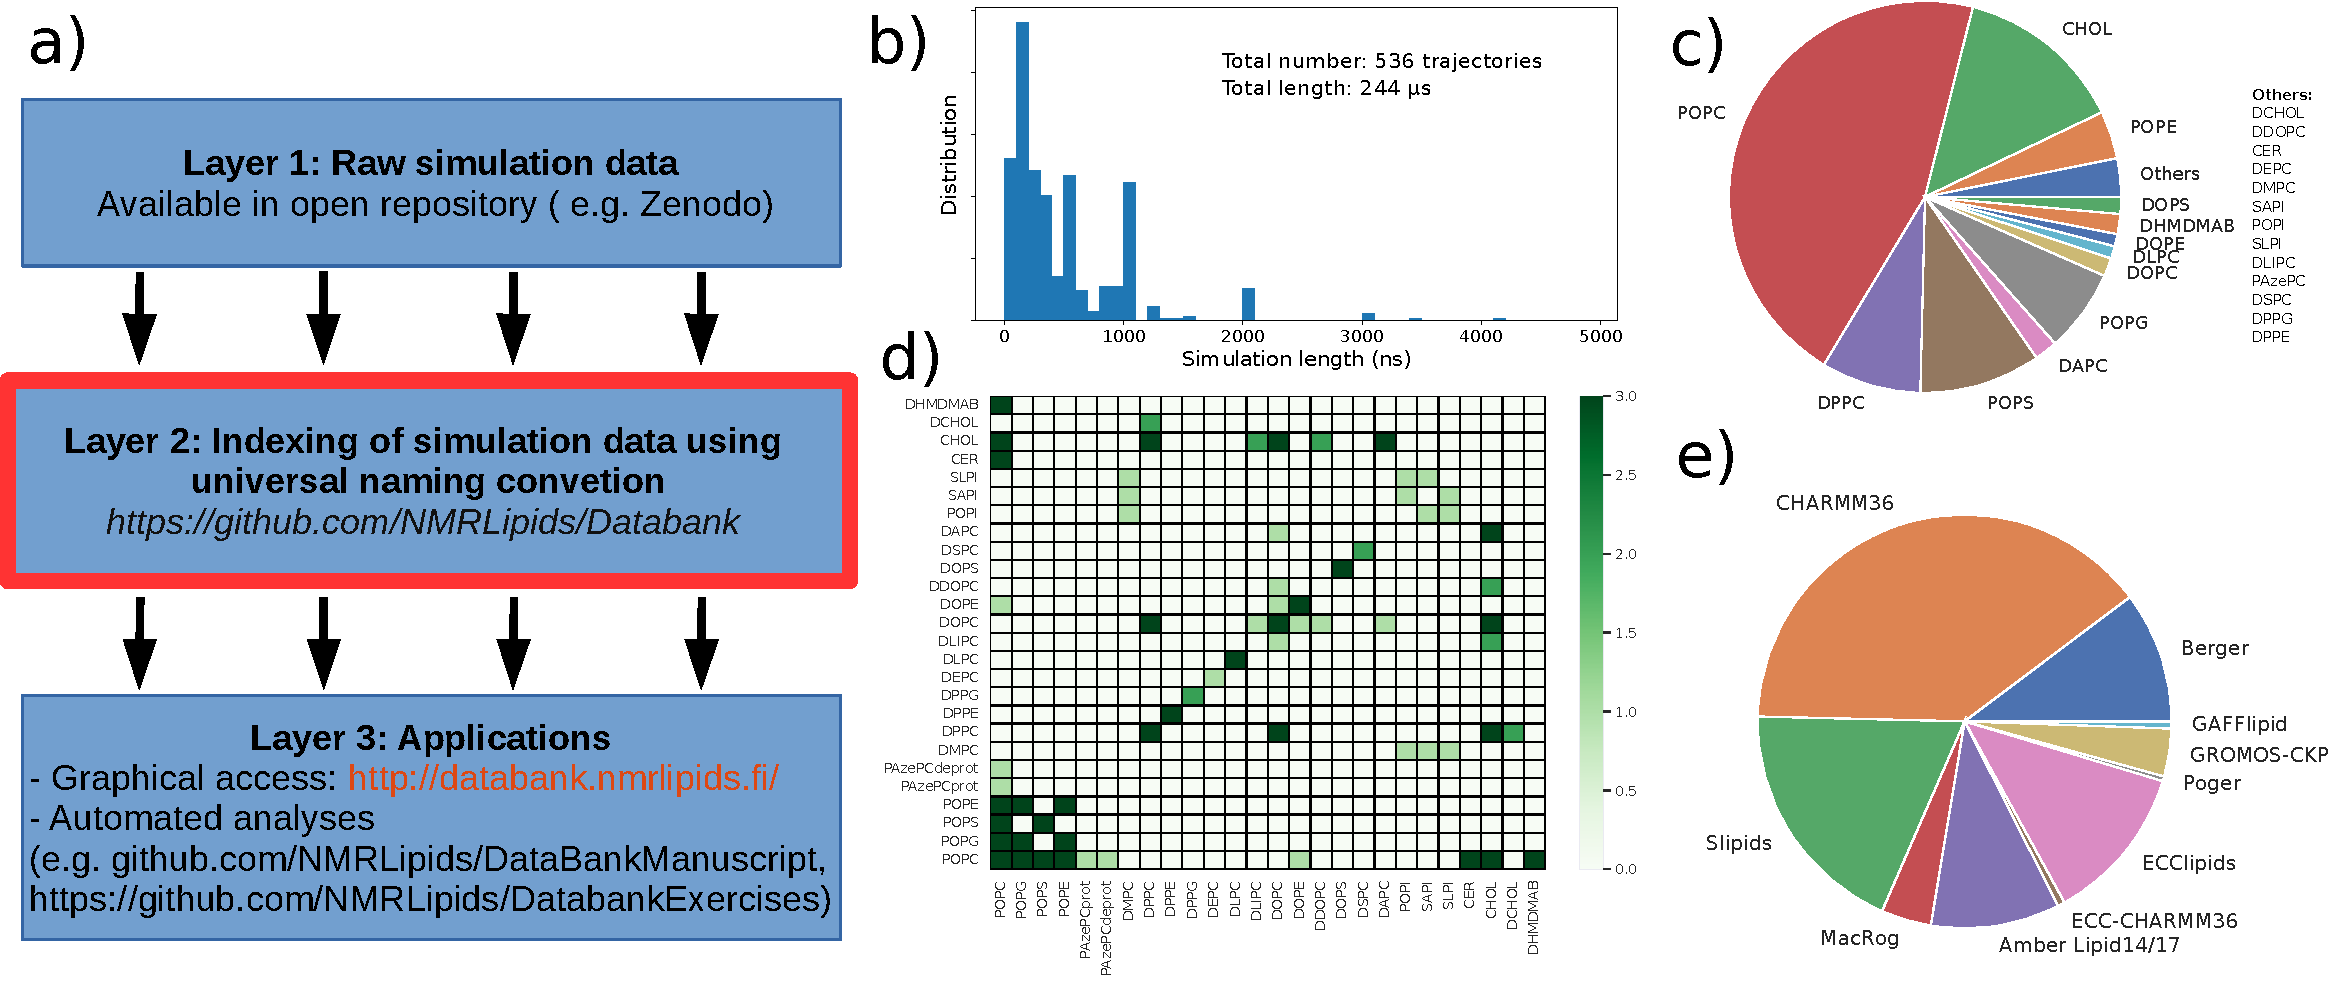
\includegraphics[width = 89mm]{Figures/overlay.pdf}
    \caption{Structure of a overlay databank illustrated. 
    Raw data is available from a publicly accessible repository (layer 1).
    The core of the databank contains information on the location of the raw data and indexing of molecular compositions and simulation details described with universal naming conventions (layer 2).
    The content of databank can be viewed and analysed using external programs that automatically read the information and data from layers 1 and 2 (layer 3). Examples of such applications are the GitHub repository generating the results presented in this work and the graphical access to the databank.
    More detailed description of the databank is illustrated in Fig.~\ref{DatabankStructure} in the SI.
    }
    \label{fig:overlay}
\end{figure}

Here we present a solution for lipid bilayers based on overlay databank structure illustrated in Fig.~\ref{fig:overlay}. The key idea of the overlay databank is that the storage of raw data in layer 1 is distributed in publicly available repositories or other servers with long term stability and permanent links such as digital object identifiers. The core of the databank, layer 2, contains only information on the location and content of the raw data, thereby not requiring large resources to handle and maintain. This lowers the barrier for starting such databank as well as for long term storage. The NMRlipids databank is essentially a git repository containing information on the location of raw data and its indexing with universal naming convention. In addition to all computers where the databank is developed and used, the NMRlipids databank git is stored to Zenodo server, thereby enabling a very cost effective long term storage for the databank. The databank can be used in layer 3 by accessing the raw data and information stored in the databank by employing the universal naming conventions for atoms, molecules and simulation details. The applications can be linked to the core databank (layer 2) without actually including them, thereby enabling flexible extension of the data without compromising the simplicity and lightness of the core databank. The concept of overaly databank is developed here to solve the practical challenges in generating databanks of MD simulation data enabling flexible analyses over large sets of simulation data, but it pontentially used for wide range of situations, particularly when storage of raw data requires significant resources and final outcomes or best practices are not yet clear, overlay databank approach lowers the barrier to start without compromizing the long term stability or scalability.

The practical relevance of the NMRlipids databank is exemplified by automatic quality evaluation and ranking of large amount of MD simulation data, data-driven analysis detecting correlations between properties of model cell membranes and analyses of rare phenomena that are beyond the scope of standard MD simulation studies. The NMRlipids databank provides new tools for researchers in wide range of fields in academia and industry from cell membrane biology to lipid nanoparticle formulations and data-driven computational chemistry and machine learning. 

%The Introduction section, of referenced text\cite{Figueredo:2009dg} expands on the background of the work (some overlap with the Abstract is acceptable). The introduction should not include subheadings.

\section{Results}

%Up to three levels of \textbf{subheading} are permitted. Subheadings should not be numbered.

\subsection{Quality evaluation of force fields}
Even though the quality of force fields has been widely evaluated against experimental data during parameterization and in separate comparison studies~\cite{botan15,ollila16,catte16,pluhackova16,perez17,leonard19}, defining unambiguously their overall quality still remains unclear, and several controversial results are reported for each in the literature~\cite{antila22b}.

The quality of MD simulations in the NMRlipids databank are evaluated against C-H bond order parameters from NMR and form factors from x-ray scattering, which can be robustly measured from lipid bilayers and directly connected to the simulation data~\cite{ollila16}. The first one is related to the conformational ensemble of individual lipids and latter to the overall structure of lipid bilayer. NMRlipids databank searches available experimental data for each simulations and, when found, defines the quality of a simualtion based on comparison against C-H bond order parameters and x-ray scattering form factors. For more details see the method section.

\begin{figure}
    \centering
    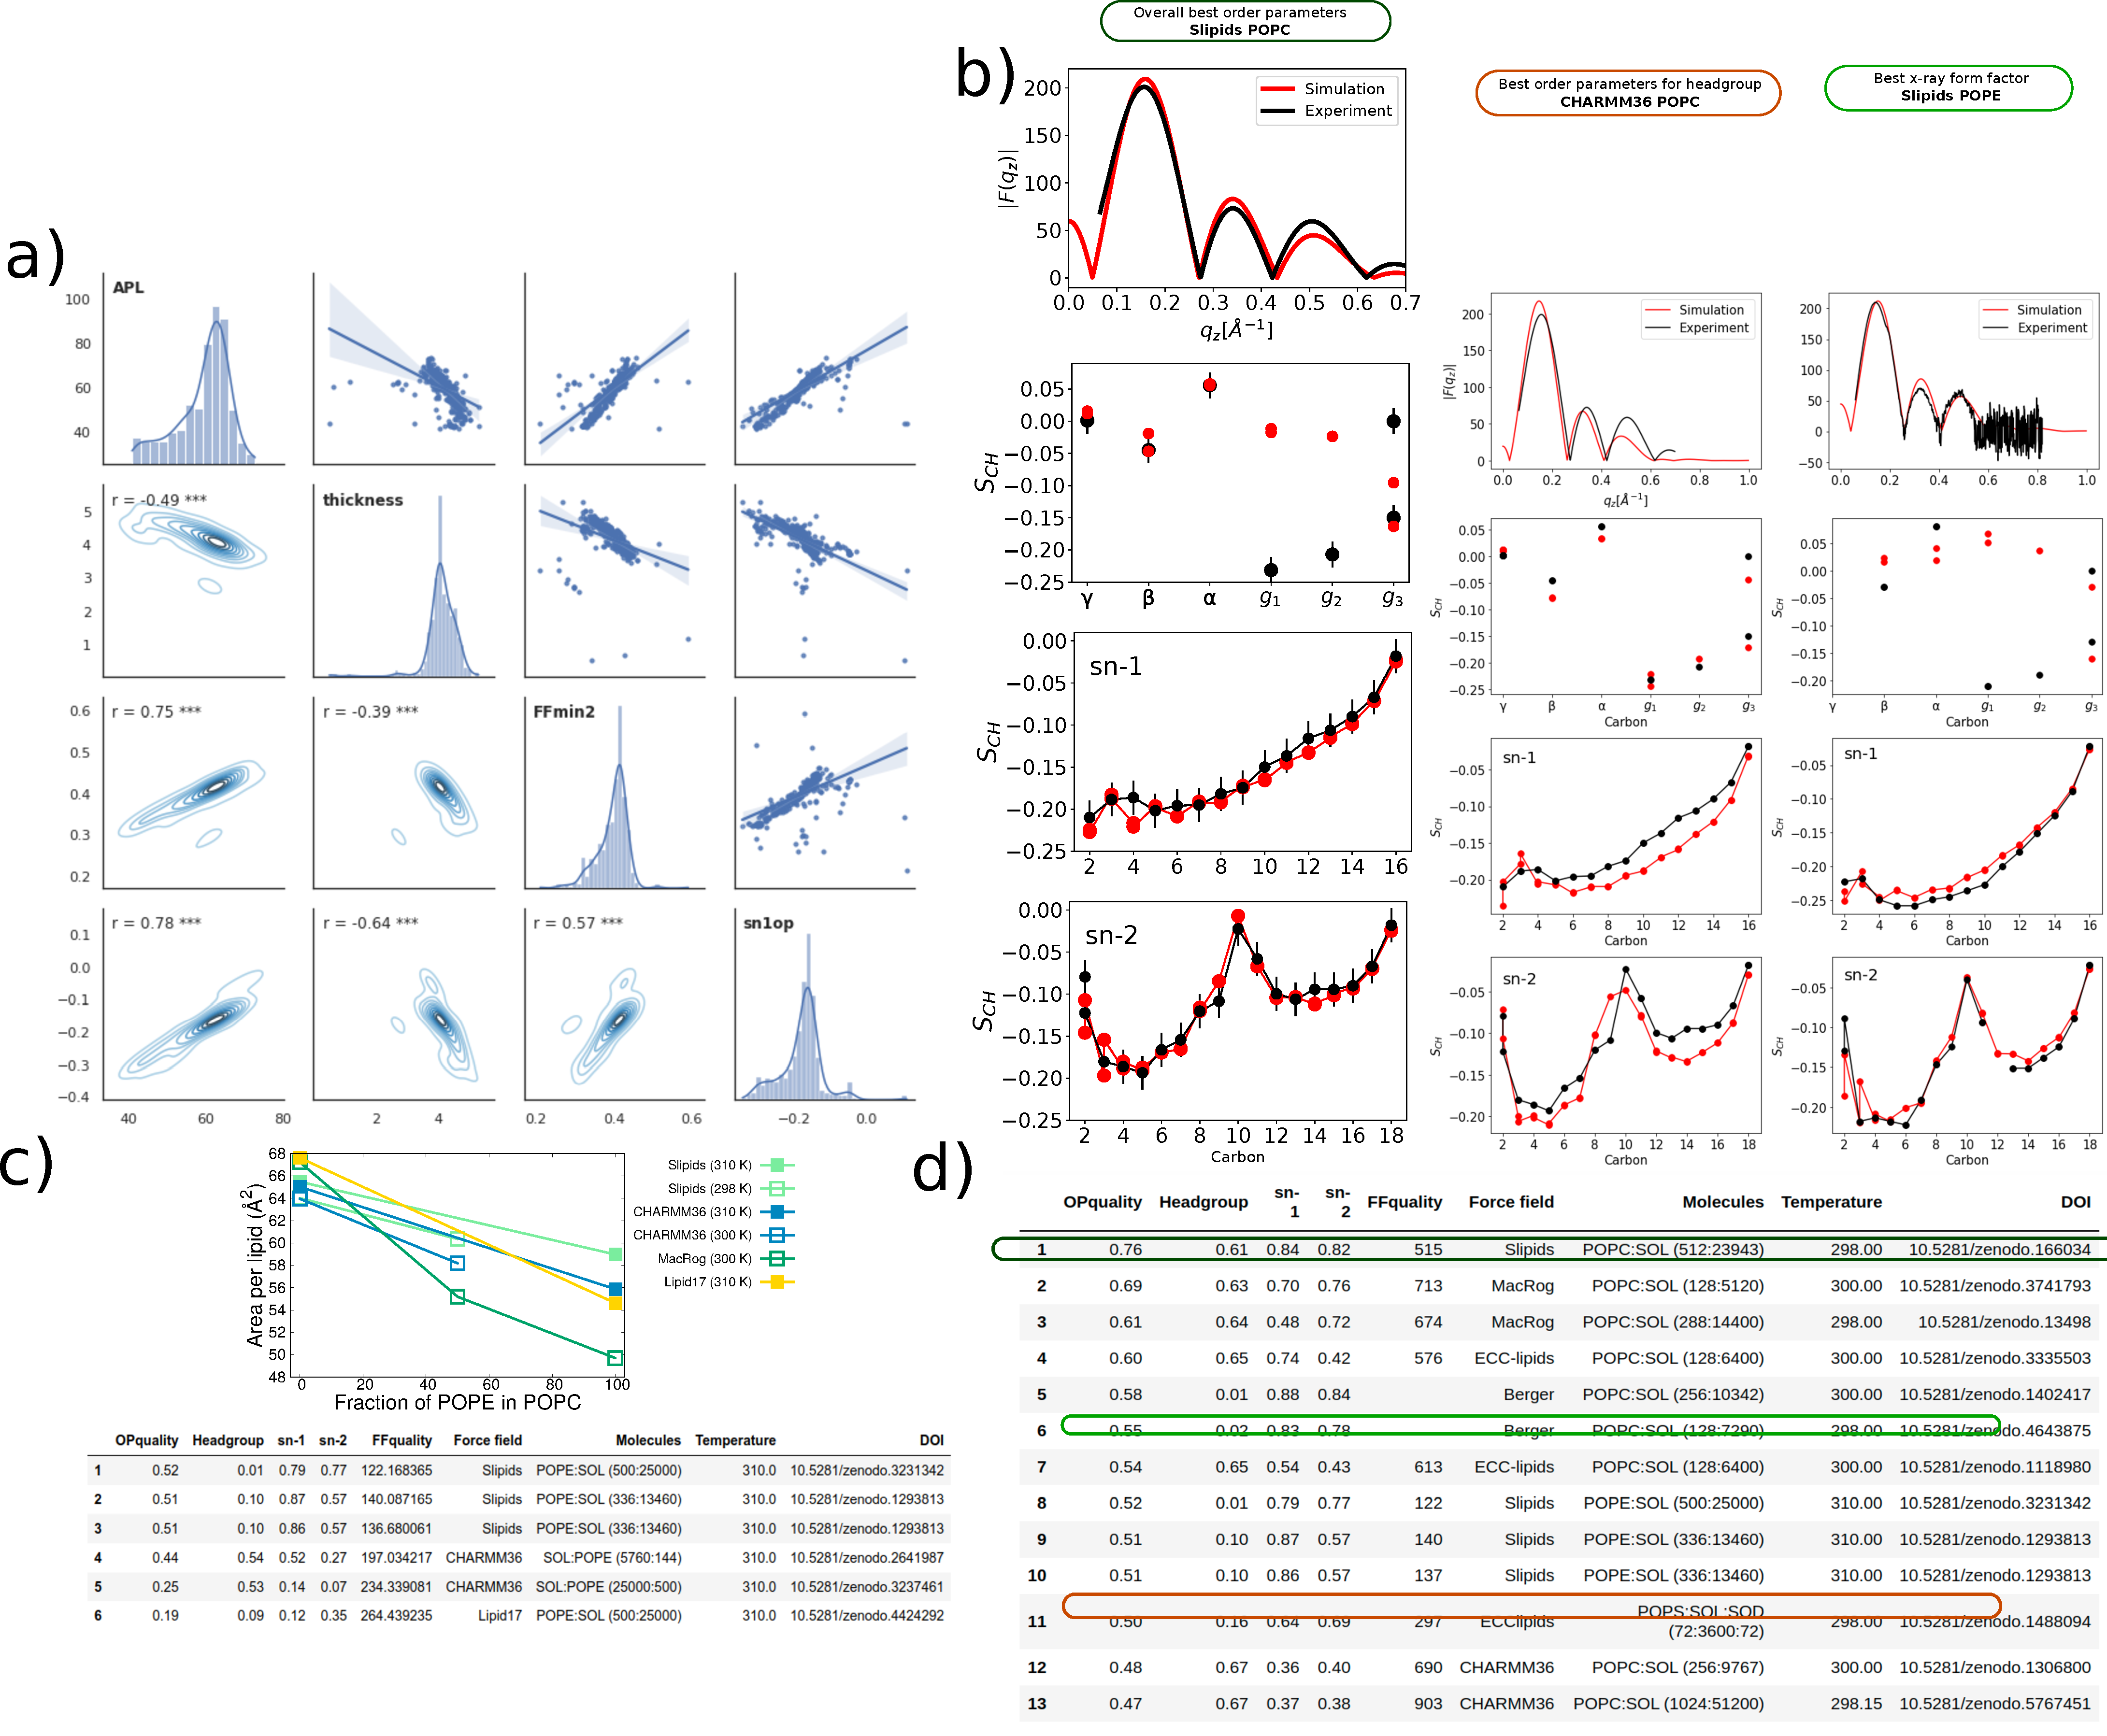
\includegraphics[width=180mm]{Figures/quality.pdf}
    \caption{Caption}
    \label{fig:quality}
\end{figure}

The top ranking simulations according to the NMRlipids measures are shown in Fig.~\ref{fig:quality}. The overall best ranking simulation, POPC lipid bilayer simulated with Slipids force field, gives a good agreement with experiments for all C-H bond order parameters except for glycerol backbone. The best simulation for headroup and glycerol backbone, CHARMM36 POPC, predicts too ordered acyl chain, thereby not being within the top 10 simulations in the overall ranking. The best ranking for x-ray form factor is given by the Slipids POPE simulation, however, because the quantitative value for form factor quality depends on the quality of experimental data, form factor qualities can be compared only between simulations evaluated against the same experimental dataset.

\subsection{Water permeability across membranes}

Averaging water density profiles over all simulations in the databank enables us to calculate the barrier for the water penetration through lipid bilayers.

\subsection{Spin relaxation rates of confined water close to membranes}

Usefulness of the databank beyond MD simulation experts is demonstrated by analysing water spin relaxation times close to bilayers which are used in MRI imaging.

%Example text under a subsection. Bulleted lists may be used where appropriate, e.g.

%\begin{itemize}
%\item First item
%\item Second item
%\end{itemize}

%\subsubsection*{Third-level section}
 
%Topical subheadings are allowed.

\section{Discussion}

%The Discussion should be succinct and must not contain subheadings.

\section{Methods}

%Topical subheadings are allowed. Authors must ensure that their Methods section includes adequate experimental and characterization data necessary for others in the field to reproduce their work.

\subsection{Structure of the databank}

\begin{figure}
  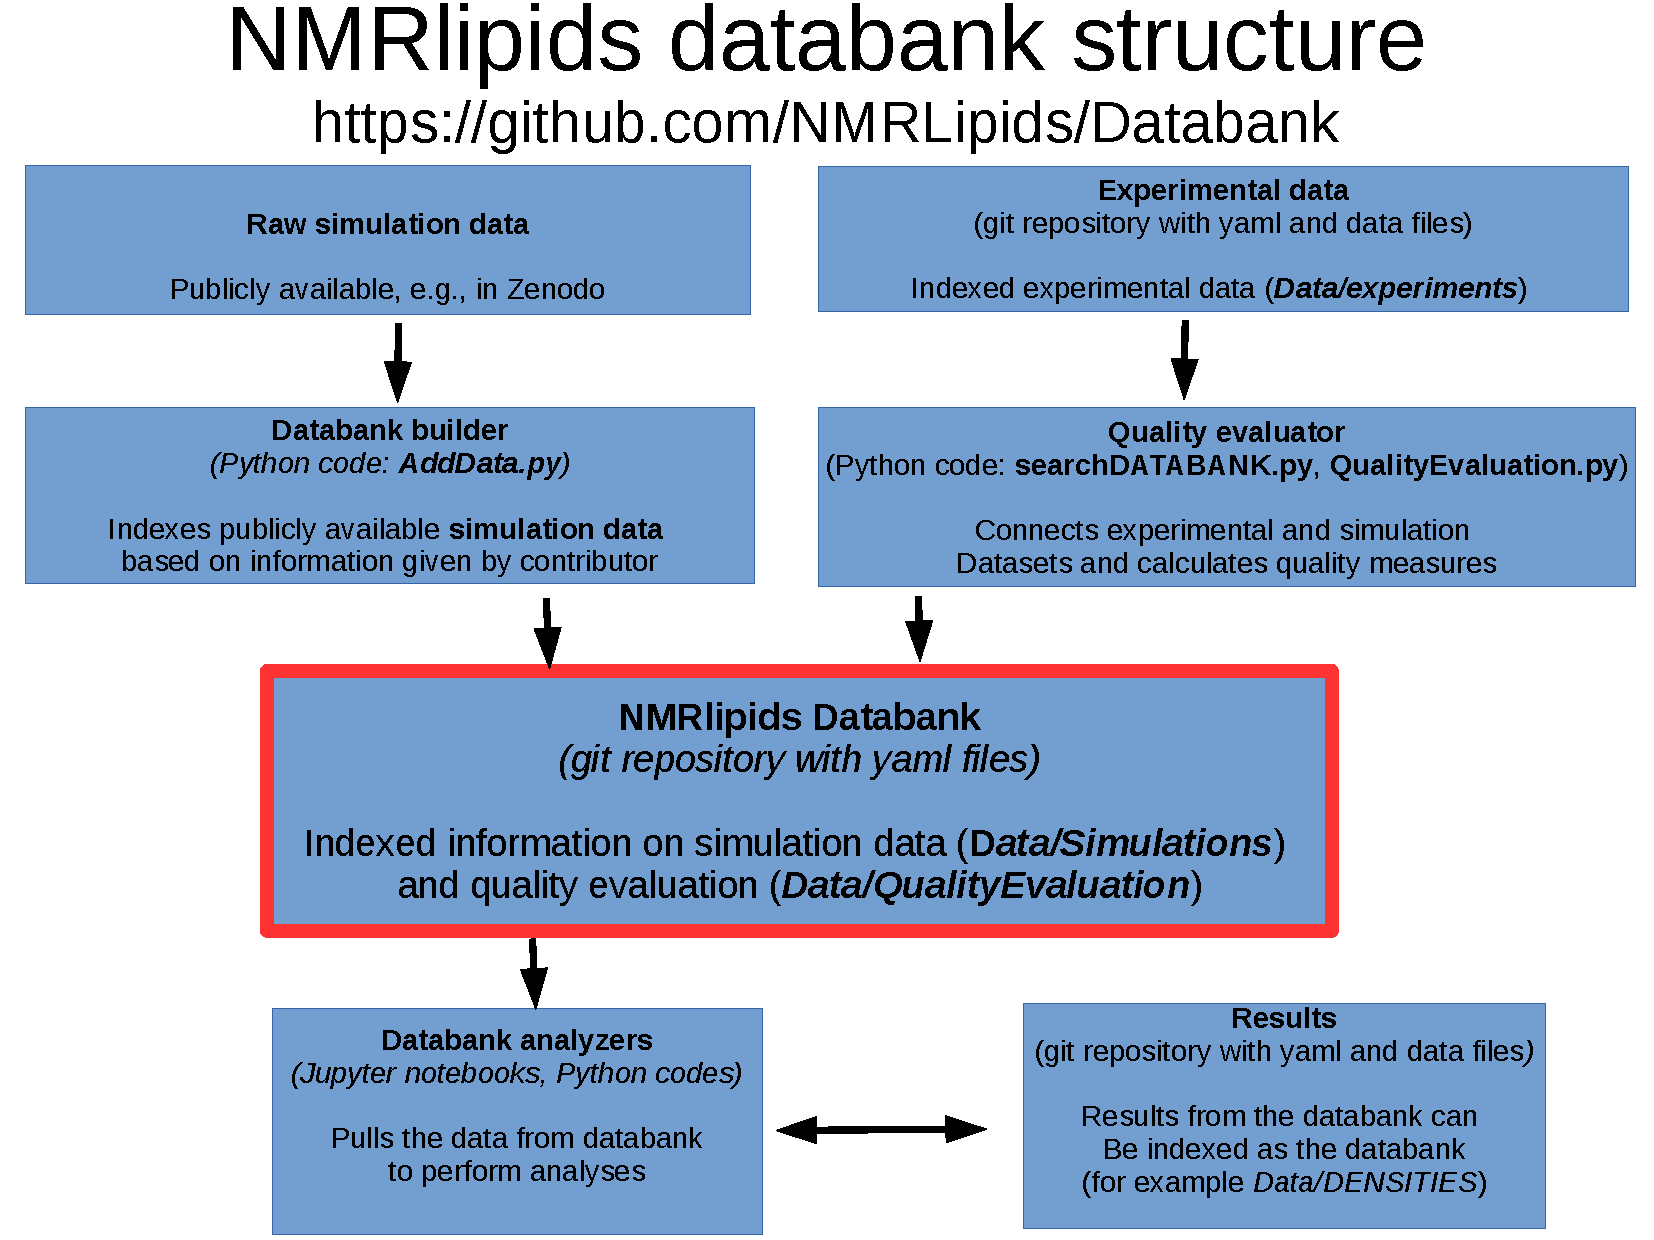
\includegraphics[width=\textwidth]{figures/DataBankStructure.pdf}
  \caption{Structure of the NMRlipids databank}\label{DatabankStructure}
\end{figure}

NMRlipids databank is a overlay databank composed of files that contain all the essential information
on the molecular dynamics simulation trajectories that are listed in the databank.
The location publicly avaiable raw MD simulation data is flexible.
The NMRlipids databank files contain all the essential information on the
original data that enable wide range of applications.
%and all essential information on simulations needed in further use and automatic analysis.

Each simulation system is identified using the hash of original trajectory and topology file. The index files are stored in folder structure based on the identity codes of the simulations.


\subsection{Quality evaluation}

For quality evaluation, each simulation is connected to a experimental dataset is similar conditions. Currently experimental and simulation datasets are paired if molar concentrations of all molecules are within $\pm$5 percentage units, charged lipids have the same counterions, and temperature is within $\pm$2 degrees. If lipid to water ratio is above ??, the systems are considered fully hydrated. Otherwise also hydration level is considered.

Quality of lipid conformational ensembles are evaluated against C-H bond order parameters from NMR experiments~\cite{ollila16}. As a first step, the quality of each order parameter is evaluated using the negative logarithm of probability to find the simulated order parameter within the experimental error bars
\begin{equation}
    S_q = -\log_{10}(P),    
\end{equation}
where the probability is calculated from the normal distribution
\begin{equation}\label{gaussian}
    P = \int_{S_{\rm exp}-\Delta S_{\rm exp}}^{S_{\rm exp}+
    \Delta S_{\rm exp}}  \frac{1}{\sigma \sqrt{2\pi}} e^{-\frac{1}{2}(\frac{x-\mu}{\sigma})^2} {\rm d}x.
\end{equation}
$S_{\rm exp}$ and $\Delta S_{\rm exp}$ are experimental order parameter and its error, and $\mu$ and $\sigma$ are the mean order parameter and its standard deviation from simulations. The quality measure $S_q$ approaches to zero when probability for agreement between simulation and experimental results approach one, and increases when simulated and experimental values diverge. The accuracy of $\pm$0.02 is currently assumed for all experimental order parameters~\cite{ollila16}. Because phospholipids sample their conformational ensemble within nanosecond timescale~\cite{ferreira15}, all simulations in the databank would be sufficiently long to sample the realistic conformational phase of individual lipids. However, some force fields exhibit too slow dynamics which leads to large error bars in order parameter values~\cite{antila21a}. Because large error bars widen the gaussian distribution in Eq.~\ref{gaussian} thereby artificially increasing the probability to find the simulated value within experimental error bars, the order parameters with error bars larger than the experimental error 0.02 are not included in the quality evaluation.

The quality of separate fragments in each lipid type within a simulation are then evaluated by averaging individual order parameter qualities over C-H bond belonging to that fragment and dividing this with the percentage of order parameters for which the quality is available within the fragment, $p$
\begin{equation}
    S_q^{\rm frag}[{\rm lipid}] = \frac{\langle S_q[{\rm lipid}]\rangle_{\rm frag}}{p_{\rm frag}[{\rm lipid}]},
\end{equation}
 where frag can be {\it sn}-1, {\it sn}-2, headgroup or total (all order parameters within a molecule). The overall quality of different fragments in a simulation are then defined as a molar fraction weighted average over different lipid components
\begin{equation}
    S_q^{\rm frag} = \sum_{\rm lipid} \chi_{\rm lipid} \langle S_q^{\rm frag}[{\rm lipid}]\rangle_{\rm lipid} ,
\end{equation}
where $\chi_{\rm lipid}$ is the molar fraction of a lipid in the bilayer.

Qualities of form factors were evaluated with the same approach that was used in SIMtoEXP program~\cite{kucerka10}. Because experiments give form factors only in relative scale those were scaled to the simulation data with absolute scale using equation
\begin{equation}
    k_e = \frac{\sum_{i=1}^{N_q} \frac{|F_s(q_i)||F_e(q_i)|}{(\Delta F_e(q_i))^2}}{\sum_{i=1}^{N_q} \frac{|F_e(q_i)|^2}{(\Delta F_e(q_i))^2}}.
\end{equation}
The quality of each form factor was then calculated from the equation
\begin{equation}
    \chi^2 = \frac{\sqrt{\sum_{i=1}^{N_q}(|F_s(q_i)|-k_e|F_e(q_i)|)^2/(\Delta F_e(q_i))^2}}{\sqrt{N_q-1}},
\end{equation}
where $F_s$ and $F_e$ are form factors from a simulation and experiment, respectively, and summation goes over the experimentally available $N_q$ points. 



\subsection{Analysis of the data in databank}

Index files in the datanbank contain all the essential information to perform analyses from the simulations. Systems under interest can be selected automatically browsing the index files and filtering the desired properties. 

Analysis results can be most conveniently stored to a new datanbank with identical indexing as the original databank. The results can be then easily shared and browsed indentically to the original databank.

\subsection{Indexing the simulation data}

%\subsubsection*{AddData.py}
AddData.py is a script that builds a database that contains a dictionary file and analysis data of each simulation. The dictionary file contains information about the simulation. The script also calculates order parameters of all CH bonds of the lipids in the simulation. To add a simulation it must be first uploaded to Zenodo (www.zenodo.org). The trajectory and topology files of the simulation are downloaded to the working directory from Zenodo but these are not saved into the database. To add a simulation to the database the user has to give some essential information about the simulation. This is done by writing a info file (*INFO.yaml) which is passed to AddData.py. 
\newline \\
AddData.py requires GROMACS and MDAnalysis library to be installed.
\newline \\
Run AddData.py as follows:
\newline \\
python3 AddData.py -f exampleINFO.yaml
\newline \\
There is also a script runAddData.sh that can be used to loop over several info files to add many simulations at one go.

%\subsubsection*{Simulation dictionary}
A simulation dictionary contains information about the simulation. Some of the information is provided by the user. The numbers of lipid molecules, solvent and ions are automatically read from the files and so are the simulation temperature and trajectory length. All this information is saved to a file named README.yaml.


\subsubsection{User input}
Dictionary variables defined by the user are listed here. 
The necessary parameters required for the analyses are described first and are marked as ''compulsory''. Then the parameters used to describe the data for further usage and analyses are described.
While only compulsory parameters are required for the databank entry, strong recommendation is that all the possible parameters would be given to maximize the possibilities to upcycle the contributed data. 

\subsubsection*{DOI (compulsory)}
Give DOI identity from where the simulation files are located. Current databank works only for the data in Zenodo, but other potential sources are may be implemented in the future. Note that the DOI must point to a specific version of dataset in Zenodo, i.e., DOI pointing to all versions of certain dataset does not work.

\subsubsection*{SOFTWARE (compulsory)}
Give the name of software used to run the simulation. The options are GROMACS, AMBER, NAMD, CHARMM and OPENMM. So far, only simulations run with GROMACS are accepted by the script.

\subsubsection*{TRJ (compulsory)}
Give the name of the trajectory file that is found from the DOI given above.

\subsubsection*{TPR (compulsory)}
Give the name of the file with topology information (tpr file in the case of Gromacs) that is found from the DOI given above.

\subsubsection*{PREEQTIME (compulsory)}
Give the time simulated before the uploaded trajectory in nanoseconds. For example, if you upload 100-200~ns part of total 200~ns simulation, this should value should be 100.

\subsubsection*{TIMELEFTOUT (compulsory)}
Give the time that should be considered as an equilibration period in the uploaded trajectory. Frames before the give time will be discarded in the analysis. For example, if you upload 0-200~ns part of total 200~ns simulation where the first 100~ns should be considered as an equilibration, this value should be 100.


\subsubsection*{Molecule names (compulsory)}
In the databank, each molecule has a unique abbreviation (see table~\ref{tab:abbreviations}). 
You need to give the residue names of these molecules corresponding your simulation.
%The user must also provide the names of the molecules, ions and solvent that are used in the simulation to match the names used by the databank. The names provided by the user must be the same as in the tpr file. 
If atoms in a lipid belong to different residues (typical situation in Amber force fields), give the name of the head group residue here, and add the residue name of each atom to the third column in the mapping file (see below). If your simulation contains molecules that are not yet in the databank, you need to define the abbreviation and add molecules to the lipids\_dict, molecules\_dict, molecule\_numbers\_dict and molecule\_ff\_dict in the AddData.py script, as well as to table~\ref{tab:abbreviations}. 

\begin{table}[h]
    \centering
    \begin{tabular}{c|c}
        Abbreviation & Molecule name \\
        \hline
        POPC &  1-palmitoyl-2-oleoyl-sn-glycero-3-phosphocholine\\
        POPG &  1-palmitoyl-2-oleoyl-sn-glycero-3-phosphoglycerol \\
        POPS & 1-palmitoyl-2-oleoyl-sn-glycero-3-phospho-L-serine \\
        POPE & 1-palmitoyl-2-oleoyl-sn-glycero-3-phosphoethanolamine \\
        CHOL & cholesterol \\
        DHMDMAB & dihexadecyldimethylammonium \\
        \hline
        POT & potassium ion \\
        SOD & sodium ion \\
        CLA & chloride ion \\
        CAL & calcium ion \\
        SOL & water \\
    \end{tabular}
    \caption{Abbreviations used in the databank}
    \label{tab:abbreviations}
\end{table}

\subsubsection*{MAPPING\_DICT (compulsory)}
For the analysis, we need to know the names of atoms in your system.
These are defined using the mapping file convention introduced in \url{http://nmrlipids.blogspot.com/2015/03/mapping-scheme-for-lipid-atom-names-for.html}, where first column gives the universal atom name, second gives the atom name in force field, and third gives the residue name if not the same for all atoms.
The name of the mapping file for each molecule needs to be given in dictionary format. The dictionary the key is the molecule name (abbreviation listed in table \ref{tab:abbreviations}) and the value is the name of the mapping file. The already existing mapping files can be found from the directory named "mapping\_files". If a mapping file for your molecule(s) do not exist, you need to construct one and add to the "mapping\_files" directory.

%\newline \\
%The purpose of a mapping file is to circumvent the problem caused by different atom naming conventions used by different force fields. The first column of a mapping file contains general atom names. The second column contains the name of the atom as it is in the force field. If the lipid consists of several residues which is the case in some AMBER force fields, then a third column is needed which contains the name of the residue to which each atom belongs to.

\subsubsection*{DIR\_WRK (compulsory)}
Give the path of the working directory in your local computer. The trajectory and topology files will be downloaded to this trajectory, and temporary files created during processing will be stored here. 


\subsubsection*{UNITEDATOM\_DICT (compulsory for united atom trajectories)}
Order parameters from united atom simulations are calculated using buildH code (\url{https://github.com/patrickfuchs/buildH}). For united atom simulations, you need to tell how hydrogens are added based on definitions in the dic\_lipids.py dictionary. This is done by giving a dictionary where the key is the molecule name (abbreviation listed in table \ref{tab:abbreviations}) and the value is the correct dictionary key in dic\_lipids.py. If correct dictionary key is not yet found, you need to add to dic\_lipids.py. 
In the case of an all atom simulation, UNITEDATOM is left empty.


\subsubsection*{PUBLICATION}
Give reference to a publication(s) related to the data.

\subsubsection*{AUTHORS\_CONTACT}
Give the name and email of the main author(s) of the data.

\subsubsection*{SYSTEM}
Give description of system in free format. For example ''POPC with cholesterol at 301K''.


\subsubsection*{SOFTWARE\_VERSION}
Give the version of the software used.

\subsubsection*{FF}
Give the name of the force field used used in the simulation.

\subsubsection*{FF\_SOURCE}
Describe the source of the force field parameters. For example, CHARMM-GUI, link to webpage where parameters were downloaded, or citation to a paper.

\subsubsection*{FF\_DATE}
Give the date when parameters were accessed or created. The format is day/month/year.

\subsubsection*{Individual force field names for molecules}
In some cases special force fields are used for certain molecules. For example, non-standard parameters for ions or other molecules have been used. These can be specified giving forcefield names separately for individual molecules. These can be given as parameters named as
FF+[abbreviation from table \ref{tab:abbreviations}], i.e., FFPOPC, FFPOT, FFSOL etc.

\subsubsection*{CPT (Gromacs)}
Give the name of the Gromacs checkpoint file that is found from the DOI given above.
CPT stands for the name of the cpt file. 

\subsubsection*{LOG (Gromacs)}
Give the name of the Gromacs log file that is found from the DOI given above.

\subsubsection*{TOP (Gromacs)}
Give the name of the Gromacs top file that is found from the DOI given above.



\subsubsection{Automatically analyzed parameters}
The following parameters are read automatically from the trajectory and topology files.
%%%%%%%%%%%%%%%%%%%%%%%%%%%%automatically analyzed parameters%%%%%%%%%%%%%%%%%%%%%%%%%%%%%%
\subsubsection*{Molecule numbers}
Numbers of lipid molecules (NPOPC, NPOPG, etc.) per membrane leaflet are calculated by determining on which side of the center of mass of the membrane the center of mass of the head group of each lipid molecule is located.
\newline \\
\noindent Numbers of other molecules such as solvent and ions (NSOL, NPOT, NSOD, etc.) are read from the topology file.

\subsubsection*{Temperature}
Temperature of the simulation is read from the topology file.

\subsubsection*{Trajectory length}
The length of a trajectory is read from the trajectory file.

\subsubsection*{Date of running}
The date of running the script is saved to the README.yaml file.



\bibliography{refs.bib}

%\noindent LaTeX formats citations and references automatically using the bibliography records in your .bib file, which you can edit via the project menu. Use the cite command for an inline citation, e.g.  \cite{Hao:gidmaps:2014}.

%For data citations of datasets uploaded to e.g. \emph{figshare}, please use the \verb|howpublished| option in the bib entry to specify the platform and the link, as in the \verb|Hao:gidmaps:2014| example in the sample bibliography file.

\section*{Acknowledgements}

%Acknowledgements should be brief, and should not include thanks to anonymous referees and editors, or effusive comments. Grant or contribution numbers may be acknowledged.

\section*{Author contributions statement}

Must include all authors, identified by initials, for example:
A.A. conceived the experiment(s),  A.A. and B.A. conducted the experiment(s), C.A. and D.A. analysed the results.  All authors reviewed the manuscript. 

\section*{Additional information}

%To include, in this order: \textbf{Accession codes} (where applicable); \textbf{Competing interests} (mandatory statement). 

%The corresponding author is responsible for submitting a \href{http://www.nature.com/srep/policies/index.html#competing}{competing interests statement} on behalf of all authors of the paper. This statement must be included in the submitted article file.

%\begin{figure}[ht]
%\centering
%
\includegraphics[width=\linewidth]{stream}
%%\caption{Legend (350 words max). Example legend text.}
%\label{fig:stream}
%\end{figure}

%\begin{table}[ht]
%\centering
%\begin{tabular}{|l|l|l|}
%\hline
%Condition & n & p \\
%\hline
%A & 5 & 0.1 \\
%\hline
%B & 10 & 0.01 \\
%\hline
%\end{tabular}
%\caption{\label{tab:example}Legend (350 words max). Example legend text.}
%\end{table}

%Figures and tables can be referenced in LaTeX using the ref command, e.g. Figure \ref{fig:stream} and Table \ref{tab:example}.

\end{document}
